\section{System design} % (fold)
\label{sec:system_design}

The S7Finder system is a loosely coupled high cohesion iPad application, which is used to find
the location of employees at the Subsea7 offices. The system is highly compartmentalised, to ensure that
it is both robust and easy to maintain. Data is passed to the system from a gateway server deployed by
Subsea7. This gateway is outside of the scope of the S7Finder system, but will communicate with it using
a protocol defined in the \texttt{Parser} subsystem.

\begin{figure}[h!]
    \centerline{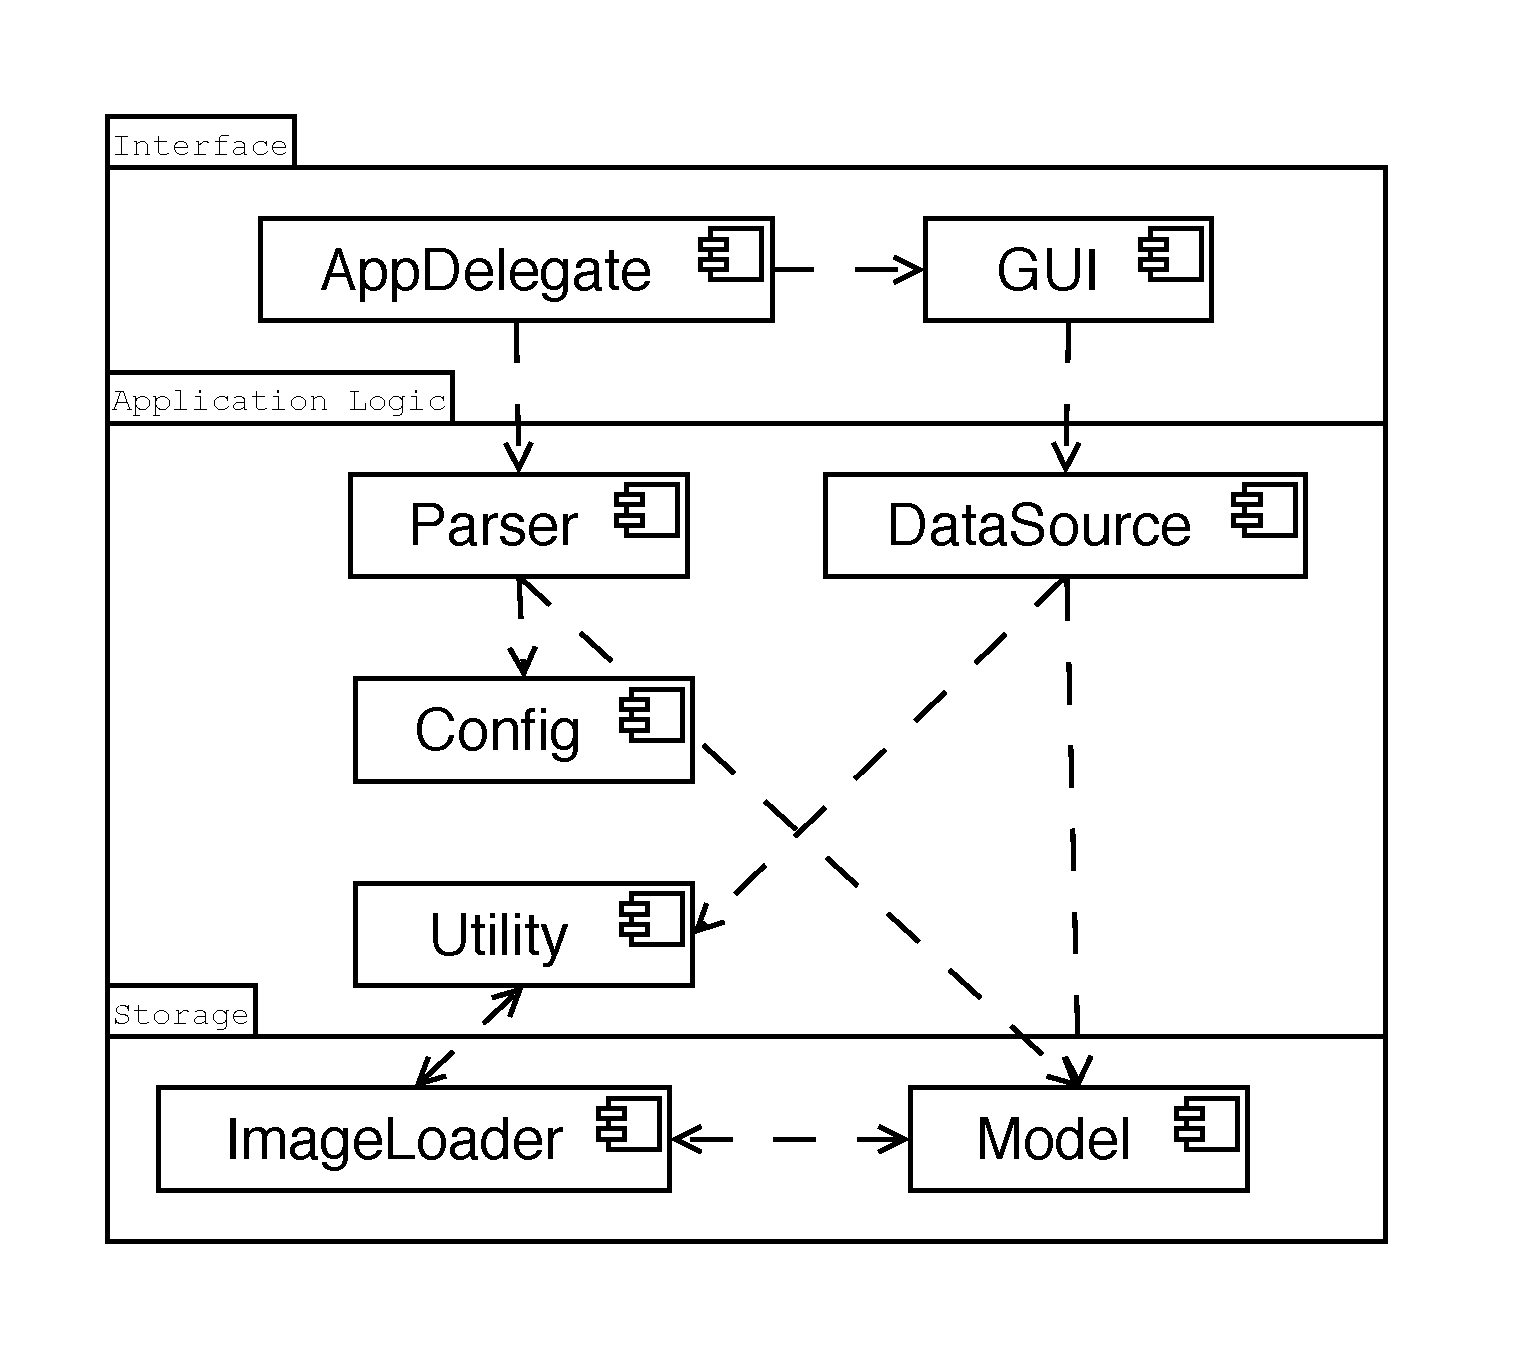
\includegraphics[width=0.75\textwidth]{system_design}}
    \caption{S7Finder subsystem decomposition}
    \label{fig:subsystem_decomposition}
\end{figure}

\begin{description}

    \item[AppDelegate] \hfill \\
        The \texttt{AppDelegate} is the standard iOS controller for system events. It ensures that the
        application listens to startup events, and that all subsystems are properly initialized.

    \item[GUI] \hfill \\
        The \texttt{GUI} subsystem handles the user interface in accordance with the principles of MVC\@.
        It uses the standard components of iOS to implement a cohesive user interface and handle the transitions
        between the different views.

    \item[DataSource] \hfill \\
        The \texttt{DataSource} subsystem handles the mapping of data from our model into
        an iOS standard format for table data. It also handles indexing and filtering based on search,
        and ensures that all functions needed for the standard GUI components are implemented and overloaded.

    \item[Model] \hfill \\
        Handles the loading of data into predefined classes to ensure that the data passed
        between the subsystems is well-formed and properly typed. The \texttt{Model} subsystem also
        holds the data in memory  to ensure fast response times for queries. It also makes sure that no
        unnecessary or duplicate object creation is performed.

    \item[ImageLoader] \hfill \\
        Handles the asynchronous loading of image resources (employee-, location-pictures, and so on \dots)
        into the GUI tables, and ensures that they are properly cached.

    \item[Parser] \hfill \\
        This subsystem handles the parsing of a communication feed gathered from the gateway server.
        It is responsible for extracting data from this feed for the initialization and insertion of
        the employee data. The \texttt{Parser} communicates with the \texttt{Model} subsystem to
        insert this data into memory.

    \item[Config] \hfill \\
        Enforces a standard for configuration of the application that one is unable to handle
        outside of a local scope. Also handles loading and caching of the configuration settings to ensure
        a minimum of network requests.

    \item[Utility] \hfill \\
        The \texttt{Utility} subsystem contains general methods needed to solve standard iOS problems
        across the system. It holds parameters generated at runtime, such as the unique identifiers for
        the physical device. The \texttt{Utility} subsystem also handles normalization of UTF8 text to ensure
        a sane environment for searching and grouping of employee names.

\end{description}

The view and controller has been combined as one class, called a UIViewController.
Changing views is handled by a UINavigationController that manages views as a stack, so you can push
to display a new UIViewController, and pop to remove the current. The actual user interface definitions
will be created in a separate \textit{.storyboard} file. The data tables defined in our storyboard is
populated using the DataSource class, that contains implementations of the \textit{UITableViewDataSource}
interface.

% subsection Subsystem decomposition (end)

% section System design (end)
